\chapter{随机区域池化}
\label{cha:sap}

\section{引言}
\label{sec:sap:introduction}

对于机器学习算法,特征的表达~\cite{bengio2013representation}具有至关重要的作用,直接反映着对于原始数据统计分布和个体差异的理解。以物体分类为例,有效的特征表达形式,可以极大地简化后端的分类识别算法,提高物体识别率。长期以来,图像的特征提取一般是靠人工设计实现的,虽然已经提出了一些具有不变性(如大小,尺度,旋转,光照等)的特征,如SIFT~\cite{lowe1999object, ke2004pca,ke2004pca},HOG~\cite{dalal2005histograms}和LBP等,并且这些特征在图像的检测识中取得了重要的进展。但是这种设计特征的方法是很困难的,需要很多实验经验、启发,甚至于运气成分,耗时耗力。因此,基于学习的特征提取方法成为人们关注的重点,在过去的几年中,出现了很多较好的研究成果,其中卷积神经网络的研究与发展很大程度上推动了特征学习的研究进展。特别是在2012年Krizhevsky~\cite{krizhevsky2012imagenet}使用深度卷积神经网络模型,通过GPU并行训练的方式,在ImageNet ILSVRC-2010和ILSVRC-2012挑战赛夺冠之后,深度卷积神经网络迎来了一个高速发展的时期。

受生物视觉皮层通路的启发,卷积神经网络采用分层的方式进行特征提取,这也是卷积神经网络可以取得卓越识别性能的一个重要因素。最近几年,大量优秀的网络模型被学者们提出用于解决不同的问题,但是关于卷积神经网络模型的设计,仍然存在着很多尚未解决的问题。比如,如何提高一个卷积神经网络的特征表达能力,使学习到的特征具有更强的分类与识别能力;如何设计出一个通用并且有效的网络模型。本章针对上述两个问题进行了深入的研究。

众所周知,数据増广是一个简单有效提高网络识别能力和泛化能力的技巧。合理的数据増广方式,可以在保证不影响训练图像样本分布的情况下,扩展训练样本空间,增加输入图像的多样性。本章中,我们将数据増广的思想推广到特征空间,即特征层次的数据増广。因此,我们提出了一个新的池化方法,即随机区域池化(Stochastic Area Pooling,SAP),在不改变特征空间样本分布的情况下,扩展特征空间、增加特征的多样性,通过特征増广提高网络的泛化能力,使网络的特征表达能力更加鲁棒。不同于传统的池化方法在一个固定的区域进行池化操作,随机区域池化通过对池化区域进行随机的旋转、平移和缩放,在变换后的池化区域进行池化操作。Jaderberg等人~\cite{jaderberg2015spatial}提出的空间变换网络(Spatial Transformer Network)也采用了特征层的仿射变换。不同之处在于,空间变换网络的仿射变换参数通过学习的方式进行优化;而随机区域池化中变换参数由高斯概率分类随机产生,训练过程中不需要进行优化学习。Jaderberg等人引入一个额外的空间变换网络,通过学习的方式对其进行优化求解,最终生成具有旋转、缩放不变性的特征,整个过程需要学习大量的额外参数,计算量较大。本章提出的随机区域池化通过对特征层进行数据増广,提高网络的泛化能力,基本不会引入额外的网络参数与计算量。

同时,为了避免网络在设计过程中出现表达瓶颈问题~\cite{szegedy2015rethinking},本章提出一个通用卷积神经网络结构,如图~\ref{fig:sap_arc}所示,该结构看起来像一个倒立的T行金字塔,我们称之为T形结构。在T形结构中,与池化层直接相连的卷积层的卷积核翻倍,以此来避免池化过程中特征的过度压缩。此外,对于T形结构中的每个卷积层,我们都统一的以此采用批正则化BN,线性整流单元ReLU,和具有 0.1 丢失比率的Dropout对卷积特征进行后处理。本章所用的所有网络模型都采用了这种T型的网络结构。

本章由随机区域池化和T型结构组成的网络记为SAPNet,我们在四个图像识别数据集上对SAPNet进行了测试,在CIFAR-10~\cite{krizhevsky2009learning},CIFAR-100~\cite{krizhevsky2009learning},MNIST~\cite{lecun1998gradient}和SVHN~\cite{netzer2011reading}上,SAPNet均取得了优越的性能。本章其余内容组织如下:第~\ref{sec:sap:relate}节,回顾了与本章研究内容相关的研究工作;第~\ref{sec:sap:model}节提出了随机区域池化方法和T形网络结构的具体实现;第~\ref{sec:sap:experiment}节详细说明了SAPNet网络结构、参数设置与训练过程,对实验结果进行了必要的分析。最后,在第~\ref{sec:sap:conclude}节是对本章主要内容的总结与概括。

\section{相关工作}
\label{sec:sap:relate}

认知机(Cognitron)~\cite{fukushima1975cognitron} 和神经认知机(Neocognitron)~\cite{fukushima1980neocognitron}通常被认为是最早的卷积神经网络模型,Fukushima在神经认知机计算模型中,提出了诸如卷积、池化、感受野等重要概念,一直沿用至今。1989年,误差的反向传播机制被LeCun等人~\cite{lecun1989backpropagation}引入到神经认知机计算模型中,进一步完善了该模型,衍生出如今的卷积神经网络。

池化是卷积神经网络的一个重要组成部分,它将位置相邻且语义相近的特征规约为一个特征。池化操作可以缩小隐层特征维度,从而降低卷积神经网络的计算量,此外池化在一定程度上增强特征的平移不变性。最常见的池化操作是均值池化(Average Pooling)和最大池化(Max Pooling)~\cite{weng1992cresceptron}。受生物视觉皮层中复杂细胞~\cite{weng1992cresceptron,simoncelli1998model}运行机制的启发,$L_{p}$池化~\cite{hyvarinen2007complex,bruna2013signal}具有更强的泛化能力。Yu等人受Dropout~\cite{hinton2012improving}和DropConnect~\cite{wan2013regularization}启发,提出了混合池化(Mixed Pooling)~\cite{yu2014mixed}方法,有效地结合了最大池化和平均池化两种方法,可以更加有效地解决过拟合问题。类似的,Lee等人~\cite{lee2015generalizing}提出了混合/门式最大均值池化(Mixed/Gate Max-Average Pooling),将混合池化中的随机参数变成一个可学习的参数,通过对池化函数的优化来提高池化的特征表达能力。Zeiler和Fergus~\cite{zeiler2013stochastic}提出了随机池化(Stochastic pooling)方法,根据多项式分布在池化区域内随机选取激活值,采用随机机制来克服过拟合问题。Rippel等人~\cite{rippel2015spectral}采用频率滤波的方式实现特征降维,从而提出了光谱池化(Spectral Pooling)方法。采用线性低通滤波器来实现光谱滤波。与最大池化相比,光谱池化可以保留更多的特征信息。He等人~\cite{he2014spatial}提出了金字塔池化(Spatial Pyramid Pooling,SPP)用于提出多尺度的池化特征,该池化方法对于任意大小的输入图片均可以生成固定长度的特征向量。Gong等人~\cite{gong2014multi}提出了多尺度无序池化(Multi-scale Orderless Pooling ,MOP),在不改变网络识别能力的基础上,增强网络特征不变性。此外,Pu等人~ \cite{pu2015deep}提出随机上采样(Stochastic Unpooling)方法,用于深度生成网络的特征升维。

\section{随机区域池化网络}
\label{sec:sap:model}

本节主要介绍了随机区域池化网络SAPNet的网络结构,SAPNet采用随机区域池化和三个T形结构组成,本小节将分别从这两个主要的组成结构,详细介绍随机区域池化和T形结构的主要实现。

\subsection{随机区域池化层}
\label{sec:sap:model:sap}

\begin{figure} [t]
\centering
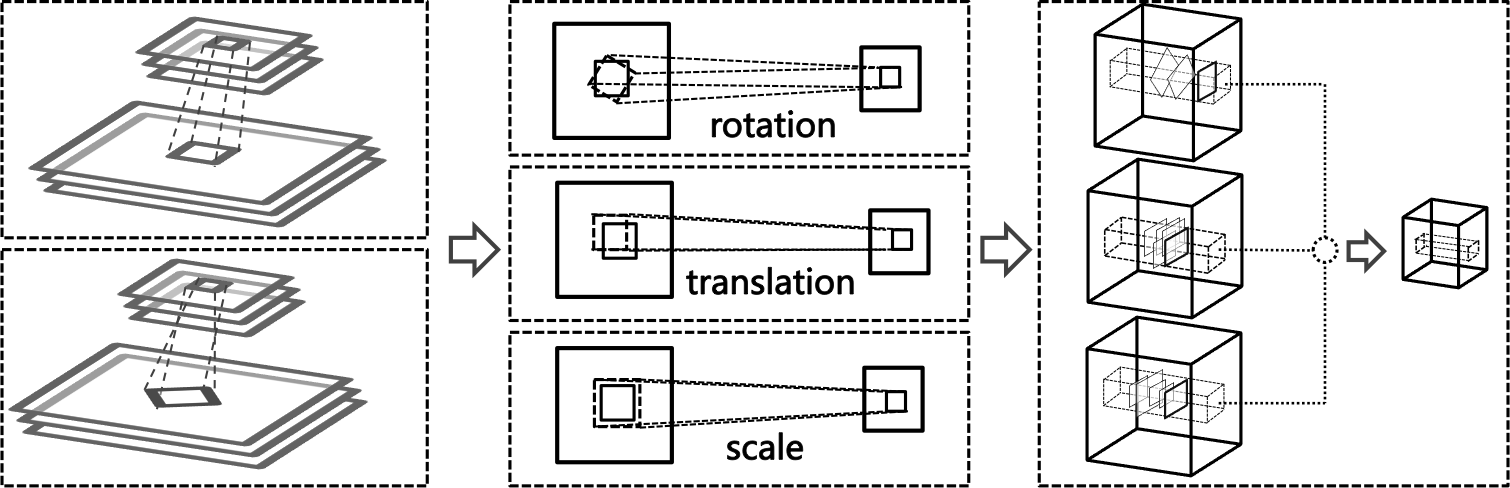
\includegraphics[width=1\linewidth]{sap_sap.png}
\caption{随机区域池化方法。}
\label{fig:sap_sap}
\end{figure}

随机区域池化主要由两个步骤组成:池化区域的选择和池化操作。首先,通过随机仿射变换对池化区域进行重采样。之后,在变换后的池化区域进行池化操作(均值池化、最大池化等),本文采用的是最大池化。

不同于传统的池化方法,在一个固定的正方形区域进行卷积操作,随机区域池化的池化区域通过仿射变换得到:$f : A {\rightarrow} B$,其中 $A {\in} \mathcal{R}^n$ 和 $B {\in} \mathcal{R}^m$ 代表两个仿射空间,假设 $x {\in} A$  代表一个 n 维向量。 仿射变换可以表示为 $f(x) = Tx + b$,其中 $T {\in} \mathcal{R}^{m \times n}$ 为仿射变换矩阵, $b {\in} B$ 为平移向量。对于二维图像空间的仿射变换,本章只考虑了最常见的平移、旋转、缩放变换和它们之间的相互组合形式,用于生成随机区域变化的池化区域。

假设 $\theta$ 代表旋转角,以向量 $[c_x, c_y]$ 为旋转中心, $[o_x, o_y]$ 平移向量,$[s_x, s_y]$ 为缩放因子。 我们可以用一个七元组 $\{\theta, c_x, c_y, o_x, o_y, s_x, s_y\}$ 来表示此仿射变换:
\begin{equation}  \label{equ:all}
  \left[
  \begin{array}{c}
          x' \\
          y' \\
          1
 \end{array}
 \right]
 =
  \left[
  \begin{array}{ccc}
          s_x \cos{\theta} & s_y \sin{\theta} & t_x\\
          -s_y \sin{\theta} & s_x \cos{\theta} & t_y\\
          0 & 0 & 1
  \end{array}
  \right]
  \left[
  \begin{array}{c}
          x \\
          y \\
          1
  \end{array}
  \right]
\end{equation}
\begin{equation} \label{equ:tx}
t_x = c_x (1 - s_x \cos{\theta}) - c_y s_y \sin{\theta} + o_x
\end{equation}
\begin{equation} \label{equ:ty}
t_y = c_x (1 + s_y \sin{\theta}) - c_y s_x \cos{\theta} + o_y
\end{equation}

随机的池化区域通过对上述七元组的随机初始化得到,七元组中每个参数服的概率分布如下:
\begin{equation} \label{equ:theta}
\theta \sim N(0, \sigma_{\theta}), 
\end{equation}
\begin{equation} \label{equ:cx}
c_x, c_y \sim N(0.5d, \sigma_{c})
\end{equation}
\begin{equation} \label{equ:sx}
s_x, s_y \sim N(1, \sigma_{s})
\end{equation}
其中 $d$ 代表输入特征图的高度或宽度;旋转角度、旋转中心、缩放因子分别服从以 0、$0.5d$、0为均值,
$\sigma_{\theta}$、$\sigma_c$ 、$\sigma_s$为标准差的高斯分布。三个标准差的大小直接影响了随机区域池化仿射变换的扰动幅度和特征増广的强度。

对池化区域进行仿射变换,变换后的池化区域往往被映射到非整数的边界上。双线性差值常用于对非整数边界上的特征值进行估计。

在每一轮前向传播的过程中,根据式(\ref{equ:theta}), (\ref{equ:cx}), (\ref{equ:sx})随机生成一组七元组参数。这组参数唯一确定了一组仿射变换的参数和变换后的池化区域,并在此区域进行池化操作,本章采用的是最大池化。反向传播的过程中,前向传播过程中随机生成的七元组和对应的池化区域保持不变,即我们并不对七元组进行参数上的学习与优化,误差按原路进行反向传播。实际上,随机区域池化只是在传统的最大池化基础上,增加了一个随机池化区域仿射变换过程。对池化区域进行随机的仿射变化,在亚像素级别对特征进行重采样,生成一组具有随机平移、旋转和缩放的特征表达,以此来达到特征増广的效果,如图~\ref{fig:sap_sap}所示。

我们仅将随机区域池化用于网络训练阶段,在测试阶段我们令${\sigma_{\theta}=0}$,${\sigma_c=0}$, ${\sigma_s=0}$,即跳过随机区域选择步骤,直接进行池化操作,测试阶段的随机区域池化与最大池化效果相同。这样的设计是为了避免测试阶段随机变量引起测试结果的不确定性。


\subsection{T形卷积网络结构}
\label{sec:sap:model:t}

\begin{figure} [t]
\centering
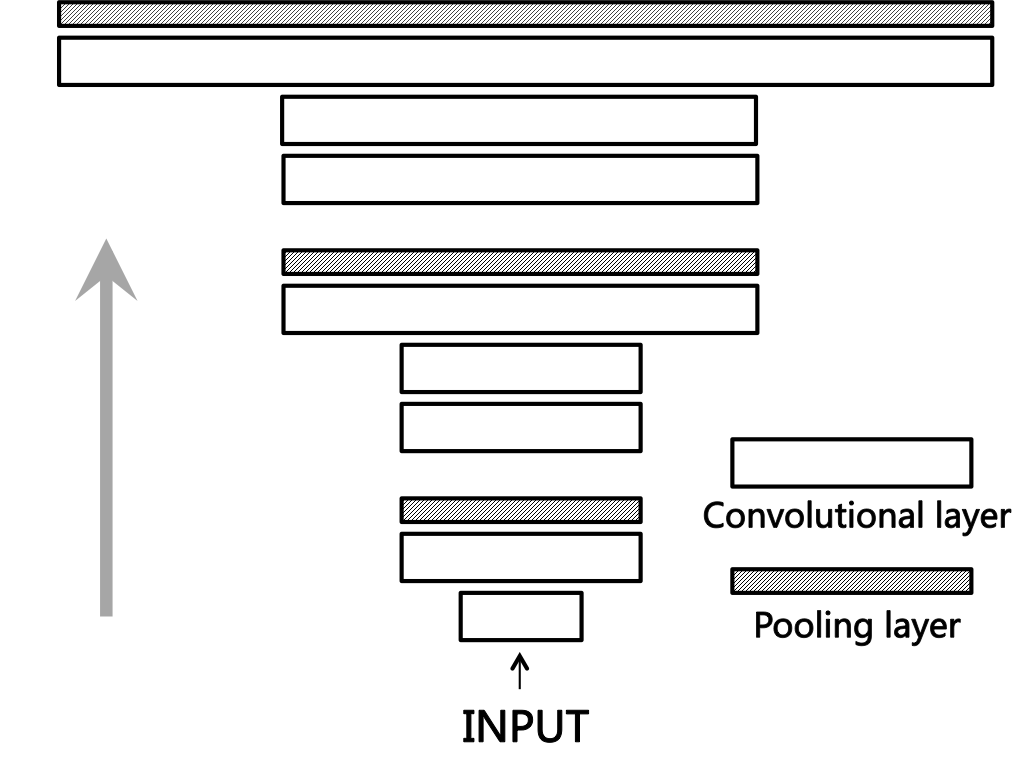
\includegraphics[width=0.7\linewidth]{sap_arc.png}
\caption{T型网络结构。}
\label{fig:sap_arc}
\end{figure}

除池化策略之外,网络结构也会影响特征表达能力。据我们了解,目前的网络结构设计还是经验主义的,并没有系统的理论支持。VGG~\cite{simonyan2014very} 和GoogLeNet~\cite{szegedy2014going,szegedy2015rethinking,szegedy2016inception}的成功启发我们,更深的网络结构、更小的感受野、合适的滑动步长均有助于网络性能的提升。最近He等人~\cite{he2015deep}的实验结果表明,随着网络深度的持续增加,识别精度会趋于饱和甚至下降。Szegedy等人~\cite{szegedy2015rethinking}同时建议,网络的设计应该避免特征表达瓶颈(Representational Bottleneck),特别在网络的初始阶段。实际上,如何确定网络的深度,保证网络的识别能力与计算复杂度;如何有效地组织卷积、池化、非线性化、Dropout层,来实现更优秀的泛化能力;如何设计每个卷积层感受野的大小和卷积核的个数,这些都是值得研究和探索的开放性问题。

\begin{table}[h]
{\caption{SAPNet 网络结构。表中一共定义四个SAPNet网络结构,SAPNet-$N$中的$N$代表与输入图像直接相连的第一个卷积层卷积核的个数。每一个SAPNet都是由三个T型结构、两个随机区域池化、一个全局均值池化、一个全连接层和一个Softmax层组成,八个卷积层被两个随机区域池化均匀隔开。}
\label{tab:model}}
\centering
\begin{tabular}{C{2.5cm}C{2.5cm}C{2.5cm}C{2.5cm}}
 \toprule[1.5pt]
\heiti{SAPNet-16} & \heiti{SAPNet-32} & \heiti{SAPNet-48} & \heiti{SAPNet-64} \\
\midrule[1pt]
conv3-16 & conv3-32 & conv3-48 & conv3-64 \\
conv3-32 & conv3-64 & conv3-96 & conv3-128 \\
\hline
\multicolumn{4}{c}{随机区域池化层} \\
\hline
conv3-32 & conv3-64 & conv3-96 & conv3-128 \\
conv3-32 & conv3-64 & conv3-96 & conv3-128 \\
conv3-64 & conv3-128 & conv3-192 & conv3-256 \\
\hline
\multicolumn{4}{c}{随机区域池化层} \\
\hline
conv3-64 & conv3-128 & conv3-192 & conv3-256 \\
conv3-64 & conv3-128 & conv3-192 & conv3-256 \\
conv3-128 & conv3-256 & conv3-384 & conv3-512 \\
\hline
\multicolumn{4}{c}{全局均值池化} \\
\hline
\multicolumn{4}{c}{全连接层} \\
\hline
\multicolumn{4}{c}{Softmax层} \\
 \bottomrule[1.5pt]
\end{tabular}
\end{table}

本节中,我们精心设计了一个通用的T形卷积网络结构,如图~\ref{fig:sap_arc} 所示。我们用长条状的立方体表示卷积层,立方体的长度代表卷积核的个数。不同于VGG结构在同一个阶段采用相同的卷积核数量进行分层的特征提取,T形结构中与池化层相连的卷积层卷积核个数会翻倍,此结构看起来像一个T型的倒金字塔,我们称之为T型网络结构。采用第~\ref{sec:sap:model:sap} 节随机区域池化和T型结构,我们构造了SAPNet,如表~\ref{tab:model} 所示。表~\ref{tab:model} 中,我们一共定义四个SAPNet网络结构,SAPNet-$N$中的$N$代表与输入图像直接相连的第一个卷积层卷积核的个数。每一个SAPNet都是由三个T型结构、两个随机区域池化、一个全局均值池化、一个全连接层和一个Softmax层组成,八个卷积层被两个随机区域池化均匀隔开。第一个T型结构中仅包换两个卷积层,这是因为相对于其他特征层,输入图片的尺寸最大,出于减少计算量的角度考虑,在第一个T型结构中去掉了一层卷积。

在SAPNet中,所有的卷积都采用 $3\times3$ 大小的感受野,1 个像素的填充,1 个像素的卷积滑动步长,这样的配置可以保持卷积后的特征尺寸保持不变。在随机区域池化层,我们采用 $2\times2$ 的池化区域大小和 2 个像素的池化窗口滑动步长。最后一个卷积层之后,采用全局均值池化来提取固定维度长度的特征。与其他图像识别任务相似地,我们也采用Softmax层作为各类别的预测概率。此外,对于所有的卷积层,我们依次采用批正则化BN~\cite{ioffe2015batch}对特征进行正则化处理,线性整流单元ReLU作为非线性激活函数,具有 0.1 丢弃率的Dropout来防止网络过早的进入过拟合。本章采用的BN操作与原论文~\cite{ioffe2015batch}的略有不同,我们忽略了原文中BN的比例和平移操作,我们仅仅将BN作为对卷积特征的一种正则化。

\begin{table*}
\centering
\caption{不同深度的卷积神经网络在CIFAR-10上的性能对比。“网络结构”是对不同卷积网络结构的缩写。 例如 '2331' 指该网络结构为 8(2+3+3)个卷积层和 1 个全连接层,被 3 个最大池化分隔成 4 个部分,每个部分具有 2,3,3 个卷积层和 1 个全连接层,最后一个池化层是全局最大池化,提取具有固定长度的特征,最后通过Softmax来预测各类别的预测概率。}
\label{tab:layers}
\begin{tabular}{C{2.8cm}|C{0.9cm}C{0.9cm}C{0.9cm}C{0.9cm}C{0.9cm}C{0.9cm}C{0.9cm}C{0.9cm}C{1.cm}}%{c|ccccccccc}
 \hline
{\heiti 层数} & 6 & 7 & 8 & 9 & 10 & 11 & 12 & 13 & 14 \\
\hline
{\heiti 网络结构} & 2221 & 2321 & 2331 & 2431 & 2441 & 2541 & 2551 & 2651 & 2661\\
\hline
{\heiti 测试误差率 (\%)} & 10.09 & 8.77 & 8.53 & 8.35 & 7.93 & \bf{7.65} & 7.86 & 7.63 & 7.77\\
\hline
{\heiti 网络感受野} &  32 & 36 & 44 & 48 & 56 & 60 & 68 & 72 & 80\\
\hline
{\heiti 参数规模 (百万)} & 0.57 & 0.61 & 0.76 & 0.80 & 0.94 & 0.98 & 1.13 & 1.16 & 1.31 \\
\hline
\end{tabular}
\end{table*}

对于网络深度的选择,我们在CIFAR-10上进行了一组实验,实验结果如表~\ref{tab:layers} 所示。如果不算全连接层,本章采用的SAPNet(如表~\ref{tab:model}所示) 网络深度为八。深度为八的网络并不是表~\ref{tab:layers} 中错误率最低的,但是综合考虑网络的识别率、计算量和参数数量,可以看出具有 8-11 层卷积的网络模型都是一个合适的选择,而八层网络具有最少的计算规模和参数数量,因此本章的大部分实验都是基于八层卷积网络模型展开的。从表~\ref{tab:layers} 我们还可以看出,网络深度的选择与网络的感受野存在一定的关系。随着网络深度的增加,网络的感受野也逐渐增大,当网络的感受野增大到输入图片的 1.5-2.0 倍的时候,网络的识别能力达到峰值。继续增加网络的深度,对网络识别能力影响不大,额外增加的计算量与可学习参数并没有带来更高的回报与收益。在CIFAR-10,CIFAR-100,MNIST和SVHN这四个数据集上,输入图像的大小为$32\times32$ 或 $28\times28$,一个 8-11 层卷积的网络模型足以获取优越的识别性能。

为了解决特征瓶颈~\cite{szegedy2015rethinking}的问题,我们通过增加特征的通道数来缓解特征尺度上的锐减。特征的维度可以表示为特征的通道数与每张特征图的分辨率的乘积。一般情况下,从输入图像到最后一个卷积层,特征的维度应该缓慢的进行缩减。也就是说,我们应该避免特征维度大幅度的急剧压缩,以防止特征信息的快速流失。考虑到池化操作不会影响特征的通道数,但会成倍缩小特征图的分辨率,如果采用步长为2的滑动窗口进行池化,特征图分辨率会减小到原来的 $1/4$。由此可见,池化很有可能会导致特征因大幅压缩而出现特征的过度流失,产生特征瓶颈问题。为了克服这个现象,我们提出了T型网络结构,通过增加与池化层直接相连的卷积层中卷积核的个数,来增加池化前特征的通道数,尽量降低池化过程中特征的信息流失。

SAPNet网络在设计的过程中,需要考虑的另一个问题是如何合理的分配网络的计算复杂度。卷积神经网络的大部分计算集中在卷积操作,而决定卷积层计算量的主要是输入特征的维度和卷积参数。在池化前后,合理的分配输入输出特征图的通道数,可以有效地平衡网络的不同阶段的计算量。

\subsection{分析与讨论}
\label{sec:sap:model:discuss}

本章我们提出了一个由随机区域池化和T形网络结构组成的SAPNet网络用于图像识别任务,该网络主要由两个随机区域池化与三个T型网络结构搭建而成。

受数据増广的启发,为了提高网络的泛化能力,我们将数据増广推广到特征层,提出了随机区域池化方法。通过随机放射变换对池化区域进行扰动,生成一组具有平移、旋转和缩放的特征表达,扩大了特征的样本空间,增加了特征的多样性。随机区域池化方法并不需要优化仿射变换参数,整个计算过程十分简单快速,并未引入过多的额外计算开销,是一种计算代价很小的提升网络泛化能力的方法。值得注意的是,随机区域池化并不是一种增强特征不变性的方法,而是通过特征増广来增强网络泛化能力,防止网络过早进入过拟合的方法。本章中采用最大池化对随机区域内的特征进行规约,相当于在最大池化的技术上,对输出特征进行了合理的扰动。同样地,均值池化也可以与随机区域选择相配合,达到特征増广的效果。

此外,我们设计T型网络结构,并以此设计了SAPNet网络。不同于其他网络模型仅仅在全连接层使用Dropout,我们在每个卷积层都采用一个丢失率较小的Dropout对特征进行正则化,防止网络过早地进入过拟合状态。实验结果表明,这样的配置可以保证网络的稳定性和泛化能力。


\section{实验结果}
\label{sec:sap:experiment}

基于caffe~\cite{jia2014caffe}深度学习框架,我们实现了本章提出的随机区域池化和T型网络模型。所有的实验都以数据并行的方式运行于具有两颗GPU核心的高性能服务器。我们在四个图像识别数据集CIFAR-10,CIFAR-100,MNIST,和SVHN上对多组不同参数大小的SAPNet进行了测试,我们在CIFAR-10数据集上,设计了更多的对比实验来验证本章随机区域池化和T型网络结构的有效性。

在所有实验中,我们批大小(Batch Size)为 96 的随机随机梯度下降算法训练网络。网络的初始学习率为 0.01,网络训练过程中学习率会逐渐减小,每次缩小为原来的 $1/10$,持续缩小3次,直到学习率降低到 1e-5。网络训练过程中,采用 0.9 的动量因子(Momentum)和 0.004 的权重衰减因子(Weight Decay )对参数进行更新。对于随机区域池化层,各参数的标准差设为$\sigma_{\theta}=5^{\circ}$,$\sigma_c=0.25d$,$\sigma_s=0.01$。采用与第~\ref{sec:sap:experiment:param}节相同的数据预处理方式,即对于每张图片,逐像素减去训练图像对应位置的像素BGR均值。

\subsection{CIFAR-10}
\label{sec:sap:cifar10}

我们首先在CIFAR-10~\cite{krizhevsky2009learning}数据集上验证随机区域池化与T型网络的有效性。CIFAR-10由 60,000 张 $32\times32$ 大小的 10 类彩色图像构成,整个数据集被平均分成 6 份,每份 10,000 张图片,其中 5 份作为训练数据,1 份作为测试数据。

\begin{table}[h]
\centering
\caption{随机区域池化与其他池化方法的对比试验。表中我们对最大池化、均值池化、随机池化进行了对比实验,结果可以看出,在网络的泛化能力上,随机区域池化 > 均值池化 > 随机池化 > 最大池化。}
\label{tab:others}
%\begin{tabular}{C{3cm}C{2cm}C{2cm}}
 \begin{tabular}{lcc}
 \toprule[1.5pt]
{\heiti 模型} & {\heiti 参数规模} & {\heiti 测试错误率(\%)} \\
\midrule[1pt]
SAPNet-32(最大池化) & 0.76 M & 8.53 \\
SAPNet-32(均值池化) & 0.76 M & 8.13 \\
SAPNet-32(随机池化) & 0.76 M & 8.50 \\
\hline
SAPNet-32(随机区域池化) & 0.76 M & \bf{7.56} \\
 \bottomrule[1.5pt]
\end{tabular}
\end{table}

\begin{table}[b]
\centering
\caption{不同参数规模下随机区域池化与最大池化性能对比。SAPNet-32(随机区域池化)的性能要好于比它的参数规模与计算量大一倍的SAPNet-48(最大池化);SAPNet-48(随机区域池化)的性能与比它的规模大近一倍的SAPNet-64(最大池化)基本持平。}
\label{tab:max}
%\begin{tabular}{C{3cm}C{2cm}C{2cm}}
\begin{tabular}{lcc}
 \toprule[1.5pt]
{\heiti 模型} & {\heiti 参数规模} & {\heiti 测试错误率(\%)} \\
\midrule[1pt]
SAPNet-32(最大池化) & 0.76 M & {8.53} \\
SAPNet-48(最大池化) & 1.71 M &{7.69} \\
SAPNet-64(最大池化) & 3.03 M & {7.01} \\
\hline
SAPNet-32(随机区域池化) & 0.76 M & {7.56} \\
SAPNet-48(随机区域池化) & 1.71 M &{7.02} \\
SAPNet-64(随机区域池化) & 3.03 M & {6.61} \\
 \bottomrule[1.5pt]
\end{tabular}
\end{table}

随机区域池化与其他池化方法的对比结果如表~\ref{tab:others} 所示。实验中,我们采用了与SAPNet-32(表~\ref{tab:model})相同的八层卷积网络结构,分别用最大池化、均值池化、随机池化来替换SAPNet-32中的随机区域池化。在没有数据増广的情况下,表~\ref{tab:others} 中所有的实验都达到了一个极高的识别率。在相同的网络结构、参数规模和计算量的基础上,随机区域池化方法明显好于最大池化、均值池化和随机池化。从本次实验的结果可以看出,对于网络的泛化能力上,随机区域池化 > 均值池化 > 随机池化 > 最大池化。由此可见,相对于最大池化、均值池化和随机池化,随机区域池化可以有效地增强网络的泛化能力,提升网络的测试性能。


\begin{table}[!h]
\centering
\caption{CIFAR-10数据集上与已有模型的对比实验。}
\label{tab:cifar10}
%\begin{tabular}{C{4.5cm}C{1cm}C{2cm}}
\begin{tabular}{L{6cm}cc}
 \toprule[1.5pt]
{\heiti 模型} & {\heiti 参数规模} & {\heiti 测试错误率(\%)} \\
\midrule[1pt]
\multicolumn{3}{c}{\heiti 没有数据増广} \\
\hline
Maxout~\cite{goodfellow2013maxout} & $>$5 M & 11.68 \\
Prob maxout~\cite{springenberg2013improving} & $>$5 M & 11.35 \\
DasNet~\cite{stollenga2014deep} &  $>$5 M & 9.22 \\
NIN~\cite{DBLP:journals/corr/LinCY13} & 0.97 M & 10.41 \\
DSN~\cite{lee2015deeply} & 0.97 M &9.69 \\
%RCNN-96~\cite{liang2015recurrent} & 0.67 M & 9.31 \\
%RCNN-128~\cite{liang2015recurrent} & 1.19 M & 8.98 \\
RCNN~\cite{liang2015recurrent} & 1.86 M & {8.69} \\
ALL-CNN~\cite{springenberg2015striving} & 1.3 M & 9.08 \\
Tree+Max-Avg~\cite{lee2015generalizing} & 1.85M & \bf{7.62} \\
\hline
SAPNet-32 & 0.76 M & \bf{7.56} \\
SAPNet-48 & 1.71 M &\bf{7.02} \\
SAPNet-64 & 3.03 M & \bf{6.36(6.50$\pm$0.14)} \\
\midrule[1pt]
\multicolumn{3}{c}{\heiti 有数据増广} \\
\hline
Maxout~\cite{goodfellow2013maxout} & $>$5 M & 9.38 \\
Prob maxout~\cite{springenberg2013improving} & $>$5 M & 9.39 \\
dasNet~\cite{stollenga2014deep} &  $>$5 M & 9.22 \\
DropConnect~\cite{wan2013regularization} & 5 networks & 9.32 \\
NIN~\cite{DBLP:journals/corr/LinCY13} & 0.97 M & 8.81 \\
DSN~\cite{lee2015deeply} & 0.97 M & 7.97 \\
%RCNN-96~\cite{liang2015recurrent} & 0.67 M & 7.37 \\
%RCNN-128~\cite{liang2015recurrent} & 1.19 M & 7.24 \\
RCNN~\cite{liang2015recurrent} & 1.86 M & 7.09 \\
Highway network~\cite{srivastava2015training} & 2.3 M & 7.54(7.72$\pm$0.16) \\
ALL-CNN~\cite{springenberg2013improving} & 1.3 M & 7.25 \\
%ResNet-20~\cite{he2015deep} & 0.27 M & 8.75 \\
%ResNet-32~\cite{he2015deep} & 0.46 M & 7.51 \\
%ResNet-44~\cite{he2015deep} & 0.66 M & 7.17 \\
%ResNet-56~\cite{he2015deep} & 0.85 M & 6.97 \\
ResNet~\cite{he2015deep} & 1.7M & {6.43(6.61$\pm$0.16)} \\
Fitnet4-LSUV~\cite{mishkin2015all} & 2.5M & 6.06 \\
Tree+Max-Avg~\cite{lee2015generalizing} & 1.85M & \bf{6.05} \\
Tuned CNN~\cite{snoek2015scalable} & 1.29M & 6.37 \\
\hline
SAPNet-32 & 0.76 M & {6.77} \\
SAPNet-48 & 1.71 M & \bf{5.92} \\
SAPNet-64 & 3.03 M & \bf{5.57(5.66$\pm$0.09)} \\
\midrule[1pt]
\multicolumn{3}{c}{\heiti 超大规模数据増广} \\
\hline
Large ALL-CNN~\cite{springenberg2014striving} & - & 4.41 \\
Fractional MP~\cite{graham2014fractional} & - & \bf{3.47} \\
 \bottomrule[1.5pt]
\end{tabular}
\end{table}

为了更直观地理解随机区域池化对网络泛化能力的提升幅度,我们进行了多组随机区域池化与最大池化的对比实验,如表~\ref{tab:max} 所示。在具有相同网络结构、参数规模和计算复杂度的情况下,随机区域池化均优于最大池化。并且一个有趣的发现是,SAPNet-32(随机区域池化)的性能要好于比它的参数规模与计算量大一倍的SAPNet-48(最大池化);SAPNet-48(随机区域池化)的性能与比它的规模大近一倍的SAPNet-64(最大池化)基本持平。由此可见,采用随机区域池化的性能提升,已经近似于为网络增加了接近一倍的额外参数与计算量所能达到的效果。


最后,我们对比了SAPNet与其他曾经在CIFAR-10上取得过优异成绩的公开模型,实验结果如表~\ref{tab:cifar10}所示。我们对三组具有不同参数规模的SAPNet进行了测试,在没有数据増广的情况下,三组模型的测试错误率均优于已有的模型。即使是参数规模最小的SAPNet-32,具有大约 0.76 M 参数,性能依然超越了Tree+Max-Avg~\cite{lee2015generalizing}的性能。SAPNet-64以6.36\%的测试错误率,在没有数据増广的情况下,在CIFAR-10数据集上取得了最好结构。为了避免单次实验的偶然性,我们对SAPNet-64重复测试了五次,以保证实验结果的可靠。


特征増广与数据増广是两个不同的概念,对于采用了随机区域池化的网络模型,数据増广依然有效,可以进一步提高网络的识别率。为此,我们增加了多组在具有数据増广情况下CIFAR-10数据集的实验结果,如表~\ref{tab:cifar10} 所示。与之前的工作~\cite{goodfellow2013maxout,springenberg2013improving,stollenga2014deep,wan2013regularization,DBLP:journals/corr/LinCY13,lee2014deeply,liang2015recurrent,srivastava2015training,springenberg2014striving}相同,我们通过随机平移和水平翻转对CIFAR-10数据集的训练图像进行数据増广。测试时,从测试图像的四角和中心分别截取 $24\times24$ 像素大小的五张图片,并对其进行水平翻转,即对一共十张图片进行测试,最终的测试结果是十张图片预测概率的均值。实验结果如表~\ref{tab:cifar10} 所示,在具有数据増广的情况下,SAPNet-64以5.57\%的测试错误率,超越了Tree+Max-Avg~\cite{lee2015generalizing}。

\begin{table}[t]
\begin{center}
\caption{CIFAR-100数据集上与已有模型的对比实验。}
\label{tab:cifar100}
\begin{tabular}{L{6cm}cc}
 \toprule[1.5pt]
{\heiti 模型} & {\heiti 参数规模} & {\heiti 测试错误率(\%)} \\
\midrule[1pt]
\multicolumn{3}{c}{\heiti 没有数据増广} \\
\hline
Maxout~\cite{goodfellow2013maxout} & $>$5 M & 38.57 \\
Prob maxout~\cite{springenberg2013improving}  & $>$5 M & 38.14 \\
DasNet~\cite{stollenga2014deep} & $>$5 M & 33.78 \\
Tree based priors~\cite{srivastava2013discriminative} & - & 36.85 \\
NIN~\cite{DBLP:journals/corr/LinCY13} & 0.98 M & 35.68 \\
DSN~\cite{lee2015deeply}  & 0.98 M & 34.57 \\
%RCNN-96~\cite{liang2015recurrent} & 0.67 M & 34.18 \\
%RCNN-128~\cite{liang2015recurrent} & 1.19 M & 32.59 \\
RCNN~\cite{liang2015recurrent}  & 1.87 M & {31.75 }\\
ALL-CNN~\cite{springenberg2013improving} & 1.30 M & 33.71 \\
Tree+Max-Avg~\cite{lee2015generalizing} & 1.76 M & 32.37 \\
ELU-Network~\cite{clevert2015fast} & 39.32 M & \bf{24.28} \\
\hline
SAPNet-32 & 0.76 M & {32.22} \\
SAPNet-48 & 1.71 M &{29.32} \\
SAPNet-64 & 3.03 M & \bf{27.59} \\
\midrule[1pt]
\multicolumn{3}{c}{\heiti 具有数据増广} \\
\hline
Highway Network~\cite{srivastava2015training} & 2.30 M & 32.24 \\
Fitnet4-LSUV~\cite{mishkin2015all} & 2.5 M & 27.66 \\
Tuned CNN~\cite{snoek2015scalable} & 1.29 M & 27.40 \\
\hline
\multicolumn{3}{c}{{\bf{Extreme}} data augmentation} \\
\hline
Fractional MP~\cite{graham2014fractional} & - & 26.39 \\
 \bottomrule[1.5pt]
\end{tabular}
\end{center}
\end{table}

值得一提的是,CIFAR-10数据集上取得的最好结果是Graham等人~\cite{graham2014fractional}提出的Fractional MP。但是Graham等人对CIFAR-10进行了超大规模的数据増广,包括输入图像的平移、旋转、水平翻转、拉伸、错切等。

\subsection{CIFAR-100}
\label{sec:sap:cifar100}

CIFAR-100~\cite{krizhevsky2009learning}是一个类似于CIFAR-10的具有 100 类物体的图像数据集。使用相同的网络结构和配置参数,在没有特征増广的情况下,我们在CIFAR-100上对SAPNet-32、SAPNet-48和SAPNet-64进行了测试,实验结果如表~\ref{tab:cifar100}所示。SAPNet-64取得了 27.59\% 的测试错误率,仅次于ELU-Network~\cite{clevert2015fast},但是我们仅使用了相对于ELU-Network网络模型8\%的参数数量。在没有数据増广的情况下,27.59\% 的测试错误率已经是CIFAR-100数据集上第二好的实验结果。

CFFAR-100数据集上,每个类别只具有500个训练样本。这样的样本数量对于大规模的卷积神经网络来说是远远不够的,较小的样本数量使得网络参数的训练不够充分,尤其是对于深层的网络参数。在参数方向传播参数更新的过程中,深层网络参数的回传梯度相对较大,使得深层网络参数更新幅度较大。而对于浅层网络由于梯度弥散的原因,回传的梯度值较小,参数的更新较为缓慢。且对于浅层网络学习的往往是图像的颜色、边缘和角点等低层特征,由于特征提取的卷积核相对较为固定。对于浅层特征,所有类别的图像均可以有效地对浅层特征参数进行更新。而对于深层的网络参数,往往需要学习相对较为复杂的纹理特征,和与具体分类类别直接相关的图像局部特征,甚至整个图片的全局特征。对于这些类别相关的网络参数的学习与更新,需要同类别大量的观测数据即训练样本,使得网络的分类器和深层参数可以学习到不同类别高层特征之间的异同。

\subsection{MNIST}
\label{sec:sap:mnist}

\begin{table}[h]
\begin{center}
\caption{MNIST数据集上与已有模型的对比实验。}
\label{tab:mnist}
%\begin{tabular}{C{4.5cm}C{1cm}C{2cm}}
\begin{tabular}{L{6cm}cc}
 \toprule[1.5pt]
{\heiti 模型} & {\heiti 参数规模} & {\heiti 测试错误率(\%)} \\
\midrule[1pt]
\multicolumn{3}{c}{\heiti 没有数据増广} \\
\hline
Maxout~\cite{goodfellow2013maxout} & 0.42 M & 0.45 \\
NIN~\cite{DBLP:journals/corr/LinCY13} & 0.35 M & 0.47 \\
DSN~\cite{lee2015deeply} & 0.35 M & 0.39 \\
RCNN~\cite{liang2015recurrent} & 0.67 M & \bf{0.31} \\
Tree+Max-Avg~\cite{lee2015generalizing} & 1.85 M & \bf{0.31} \\
FitNet-LSUV-SVM~\cite{mishkin2015all} & 0.03 M & 0.38 \\
\hline
SAPNet-16 & 0.19 M & {0.31} \\
SAPNet-32 & 0.76 M &\bf{0.29} \\
\midrule[1pt]
\multicolumn{3}{c}{\heiti 具有数据増广} \\
\hline
DropConnect~\cite{wan2013regularization} & 5 networks & 0.21 \\
MCDNN \cite{ciresan2012multi} & 35 networks & 0.23 \\
 \bottomrule[1.5pt]
\end{tabular}
\end{center}
\end{table}

MNIST~\cite{lecun1998gradient}手写体数据集相对比较简单,因此,我们从表~\ref{tab:model} 中选择了两个规模最小的网络SAPNet-16和SAPNet-32进行了测试,实验结果如表~\ref{tab:mnist} 所示。采用与CIFAR-10相同的设置参数,具有大约 0.19M 参数的SAPNet-16取得了 0.31\% 的测试错误率,该结果与具有 0.67M 参数的RCNN-96~\cite{liang2015recurrent}持平。此外,更大规模的网络模型SAPNet-32取得了 0.29\% 的测试误差。在不考虑数据増广的情况下,该结果优于其他网络模型。

MNIST数据集上的最好测试结果是0.21\%,该记录是2013年Wan等~\cite{wan2013regularization}人提出的DropConnect取得的,Wan等人采用复杂的数据増广和多模型(五个网络)平均的方法,一直保持着该项记录。

\subsection{SVHN}
\label{sec:sap:svhn}

SVHN~\cite{netzer2011reading} 的图片采集自真实环境,也是一个数字识别数据集,但是由于图像的亮度变化比较剧烈,分类和识别难度要比MNIST大很多。采用与Goodfellow~\cite{goodfellow2013maxout}类似的训练步骤,我们在SVHN数据集上,对SAPNet-32、SAPNet-48和SAPNet-64 三个具有不同参数规模的网路进行了测试,实验结果如表~\ref{tab:svhn} 所示。从实验结果可以看出SAPNet-64取得了1.71\%的测试误差率,比Tree+Max-Avg~\cite{lee2015generalizing} 低了0.02\%。

\begin{table}
\begin{center}
\caption{SVHN数据集上与已有模型的对比实验。}
\label{tab:svhn}
%\begin{tabular}{C{4.5cm}C{1cm}C{2cm}}
\begin{tabular}{L{6cm}cc}
 \toprule[1.5pt]
{\heiti 模型} & {\heiti 参数规模} & {\heiti 测试错误率(\%)} \\
\midrule[1pt]
\multicolumn{3}{c}{\heiti 没有数据増广} \\
\hline
Maxout~\cite{goodfellow2013maxout}  & $>$5 M & 2.47 \\
Prob maxout~\cite{springenberg2013improving} & $>$5 M & 2.39 \\
NIN~\cite{DBLP:journals/corr/LinCY13} & 1.98 M & 2.35 \\
DSN~\cite{lee2015deeply} & 1.98 M & 1.92 \\
%RCNN-128 & 1.19 M & 1.87 \\
%RCNN-160 & 1.86 M & 1.80 \\
RCNN~\cite{liang2015recurrent} & 2.67 M & {1.77} \\
Tree+Max-Avg~\cite{lee2015generalizing} & 4.00M & \bf{1.69} \\
\hline
SAPNet-32 & 0.76 M & {1.87} \\
SAPNet-48 & 1.71 M & {1.75} \\
SAPNet-64 & 3.03 M & \bf{1.71} \\
\hline
\multicolumn{3}{c}{\heiti 具有数据増广} \\
\hline
Multi-digit number recognition~\cite{goodfellow2013multi} & $>$5 M & 2.16 \\
DropConnect~\cite{wan2013regularization} & 5 networks & 1.94 \\
 \bottomrule[1.5pt]
\end{tabular}
\end{center}
\end{table}

\section{本章小结}
\label{sec:sap:conclude}


本章我们提出了具有T形网络结构和随机区域池化的卷积网络结构SAPNet。通过对传统池化区域进行随机仿射变换,在不影响特征空间样本分布的情况下对池化特征进行扰动,扩展特征空间,增加特征的多样性,最终达到特征増广的目的。此外,我们还提出了T型网络结构,通过增加池化层之前的特征维度,可以有效地避免特征表达瓶颈问题。最后,我们在CIFAR-10,CIFAR-100,MNIST和SVHN四个数据集上对SAPNet进行了测试,实验结果表明随机区域池化的识别能力优于均值池化、最大池化和随机池化,具有较好的泛化能力。在没有数据増广的情况下,SAPNet在CIFAR-10和MNIST上取得了最好的识别性能,在CIFAR-100和SVHN排名第二。














